
% ====================================
% chapter 2
% ====================================

\chapter{BinaryConnectによる良否判定}

\section{Neural Network}
Neural Networkとはニューロンと呼ばれる人間の脳細胞をもとに作られた数理モデルである.入力に対し重みをかけた時の出力から入力の特徴を抽出し分類問題を解く機械学習の1種である.

\subsection{Neural Networkの構造}
ニューラルネットワークはユニットと呼ばれる最小要素を持ち,それに対し複数の入力と重み,バイアスから計算結果を出力する.
これらは図\ref{fig_NN1}のような構造をしており,入力$x_i$に対し重み$w$を乗算したものにバイアス$b$を足すことで出力$y$を得る.計算式は以下のように表される.
\begin{align*}
y &= w_{1}x_{1} + w_{2}x_{2} + w_{3}x_{3} + b
\end{align*}
\begin{figure}[]
  \begin{center}
    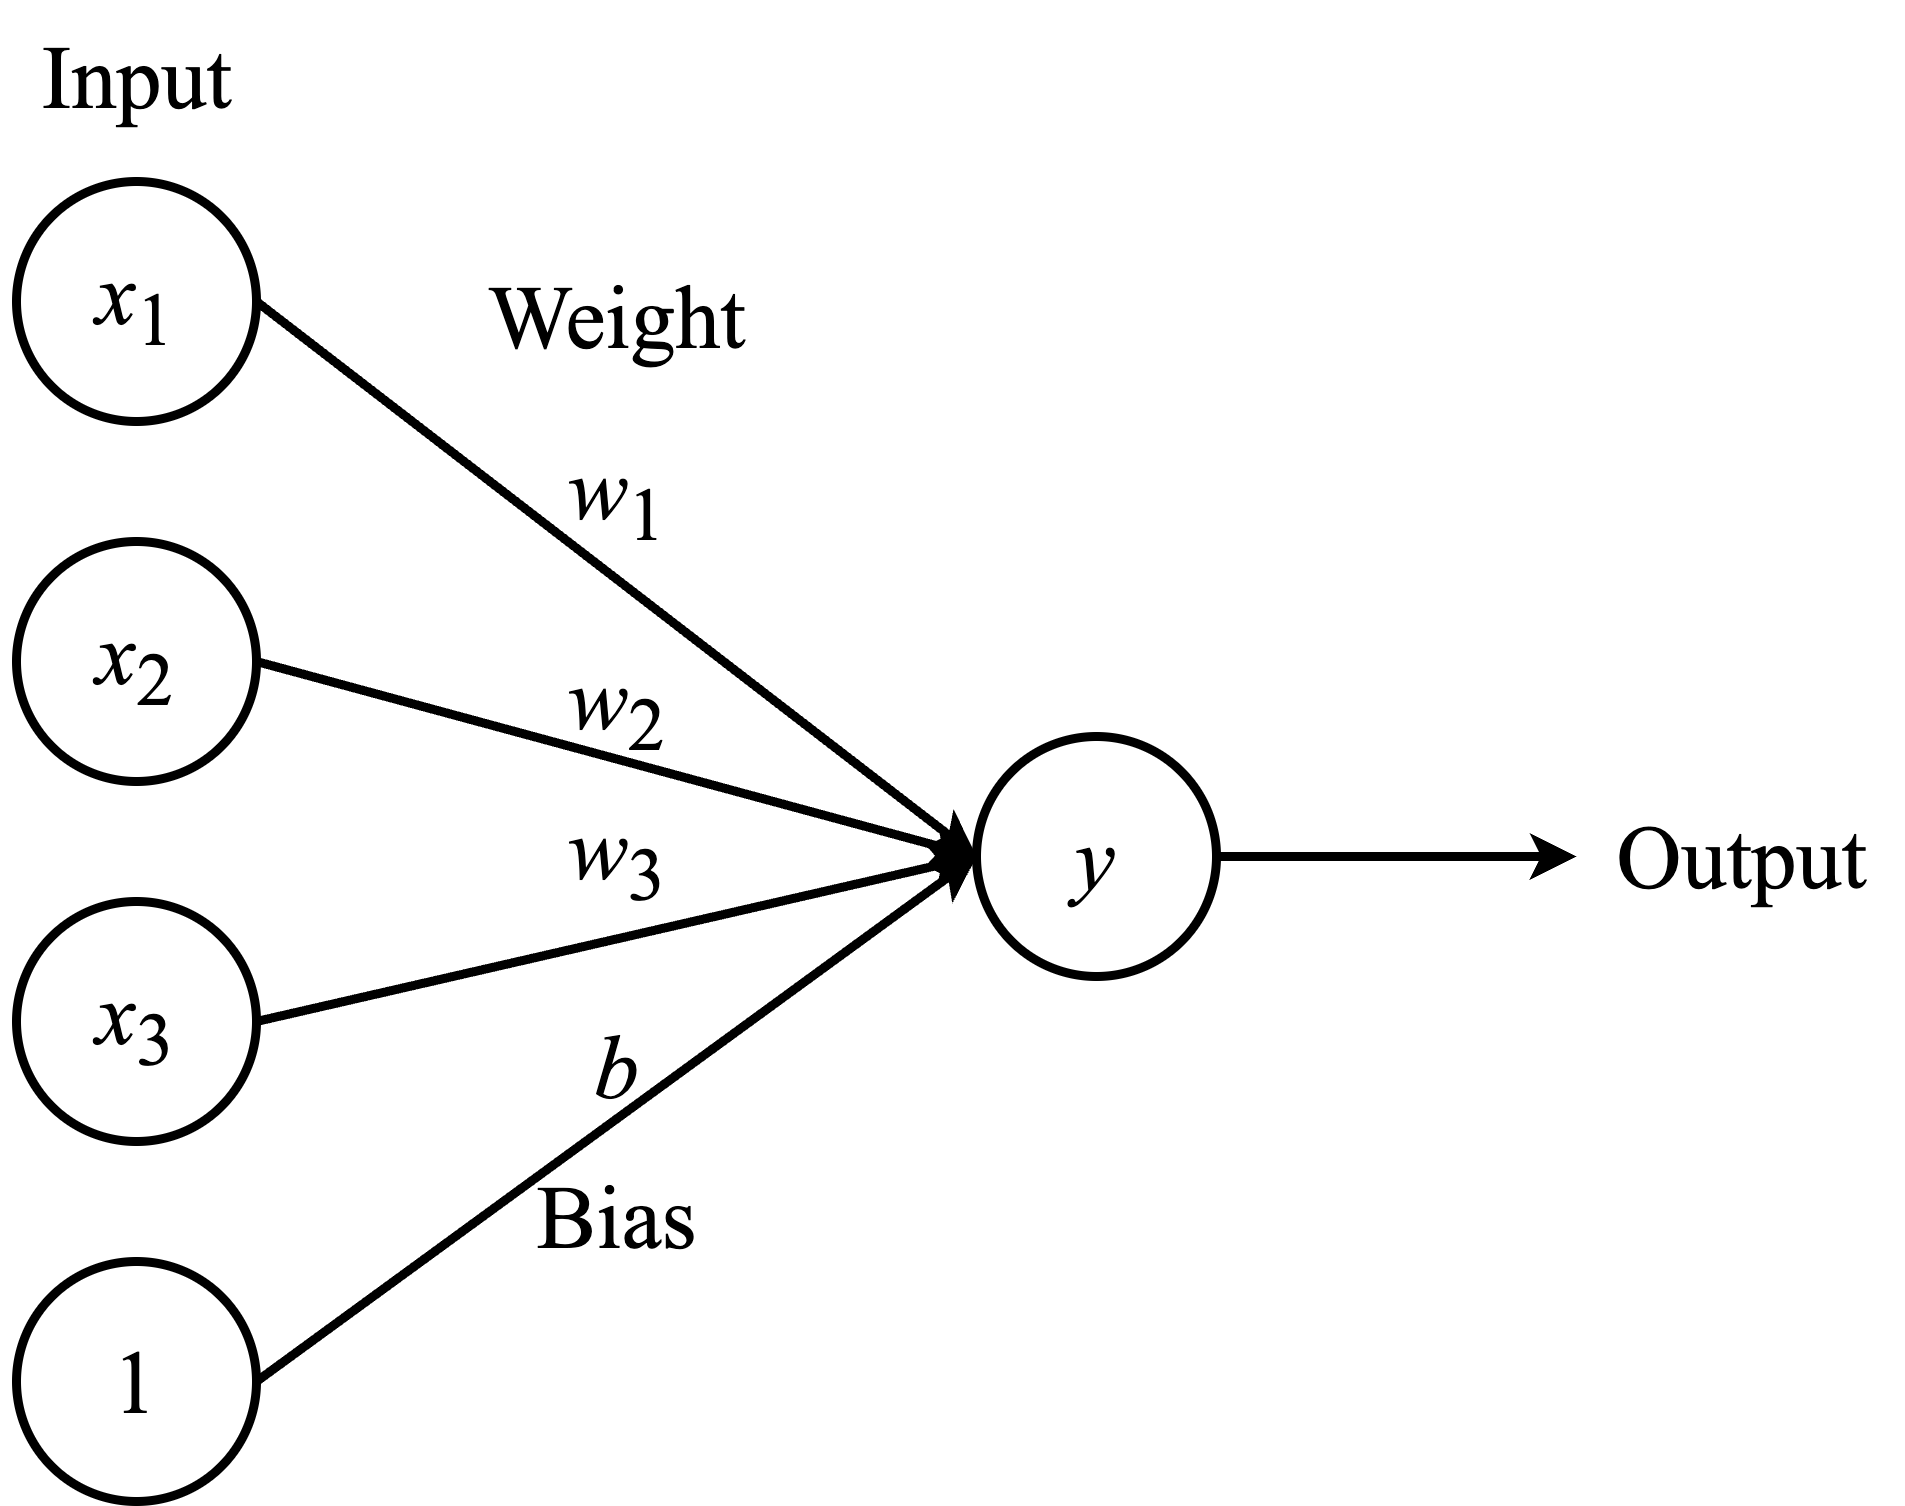
\includegraphics[scale = 0.5]{./chapter2/nn_1.pdf}
    \caption{ユニットの構造}
    \label{fig_NN1}
  \end{center}
\end{figure}

ここで出力$y$を複数個にすると,図\ref{fig_NN}のような構造になる.ユニットの縦方向の集まりのことを層(layer)と呼び,Neural Networkはこのlayerを複数組み合わせ,入力層・中間層・出力層という層を形成し計算を行う.
入力層$x$のインデックスを$i$,中間層$z$のインデックスを$j$とすると,それぞれの重みは$w_{ji}$,バイアスは$b_j$となるため計算式は以下のようになる.
\begin{figure}[]
  \begin{center}
    \includegraphics[scale = 0.5]{./chapter2/Neural_Network.pdf}
    \caption{Neural Networkの構造}
    \label{fig_NN}
  \end{center}
\end{figure}
\begin{align*}
z_{1} &= w_{11}x_{1} + w_{12}x_{2} + w_{13}x_{3} + b_1\\
z_{2} &= w_{21}x_{1} + w_{22}x_{2} + w_{23}x_{3} + b_2\\
z_{3} &= w_{31}x_{1} + w_{32}x_{2} + w_{33}x_{3} + b_3
\end{align*}

構造は学習モデルによって異なるため,必ずこのような形になるわけではない.そこで,入力の個数をI個とし,次の層のユニットへの出力を一般化すると以下のような式となる.
\begin{align*}
y_j = \sum^{I}_{i = 1} w_{ji}x_i + b_j
\end{align*}

中間層は1層のみである必要はなく,中間層の出力を次の層への入力として扱うことで層を多数化し,入力層から出力層までに多数の隠れ層を追加する.層数$L$のネットワークが存在する時,$l+1$層のユニットの出力$z^{l+1}$は$l$層のユニットの出力$z^{l+1}$から計算されるため,
\begin{align*}
  z^{l+1}_j = \sum^{I}_{i = 1} w^{l}_{ji}z^l_i + b^{l+1}_j
\end{align*}
という式で一般化される.したがって$l=1,2,3\ldots L-1$までの計算を順に行なっていくことで各層の出力を得ることができ,最終的な出力$y=z^L_j$を計算することができる.

\subsection{学習の概要}
Neural Networkでは重みを学習によって更新していく.例えば構造が図\ref{fig_NN}のような形で,出力層のユニットが2つの時は2つの分類ができユニット数が$n$個の場合は$n$個の分類ができるのである.前項のような計算をした時出力$y_1$ ,$y_2$はそれぞれ実数を持つ.これに対しSoft Max関数という活性化関数を組み込むと出力層の各ユニットに対しそのユニットが答えである確率を得ることができる.


\section{CNN}

\section{BinaryConnect}

